% lab_1.tex - Lab 1 for Cloud Computing class (Spring 2015)
% Chanmann Lim - February 2015

\documentclass[a4paper]{article}

\usepackage[margin=1 in]{geometry}
\usepackage{listings}
\usepackage{graphicx}

\begin{document}
\title{CS 7001-03: Report for Lab 1 - AWS Account Setup and Services Overview}
\author{Chanmann Lim\\ 
	\texttt{cl9p8@mail.mail.missouri.edu}}
\date{February 05, 2015}
\maketitle

\paragraph{1. } Screenshot of billing alarm setup: \\
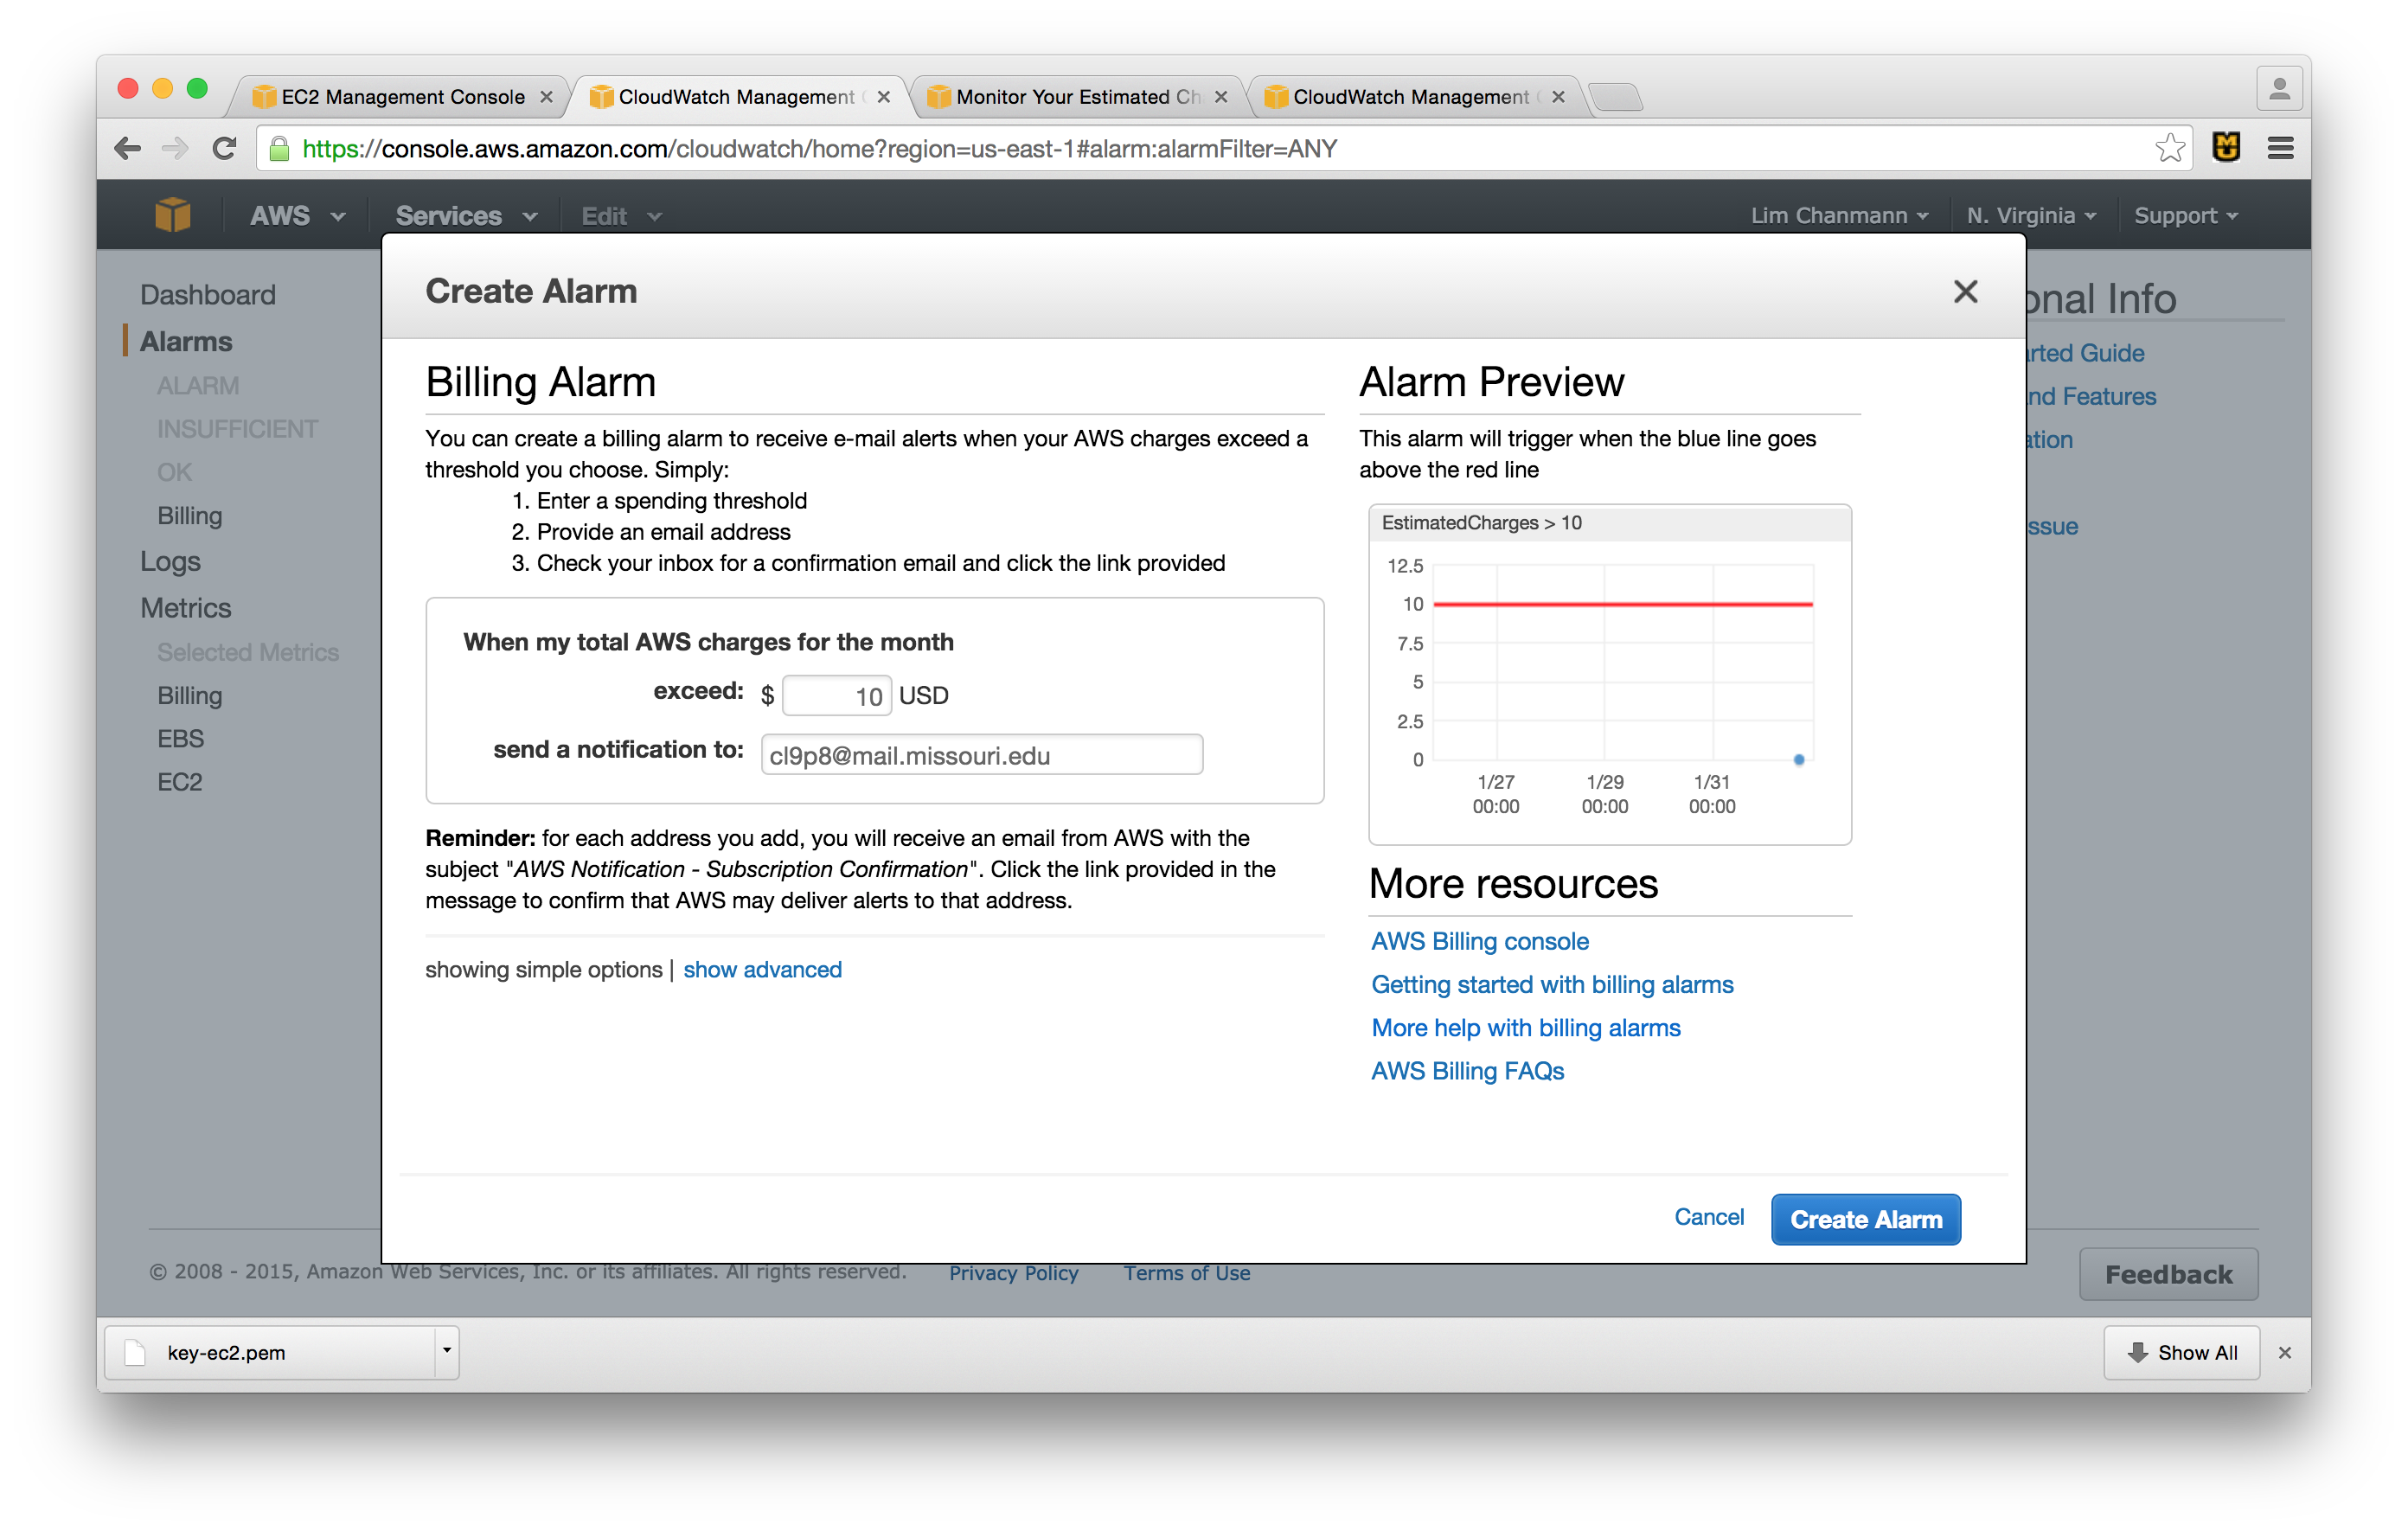
\includegraphics[scale=.32]{billing_alarm.png} \\

\paragraph{2. } List of AWS services by Categories:
\begin{description}
\leftskip 0.4in
\parindent -0.4in
	\item[Database: ] \hfill \\RDS - Relational Database Service \\DynamoDB \\ElastiCache \\RedShift
	\item[Storage \& CDN: ] \hfill \\S3 - Simple Storage Service \\Storage Gateway \\Glacier \\CloudFront
	\item[Cross-Service: ] \hfill \\Support \\Marketplace \\Managment Console \\SDKs, IDE kits and CLIs
	\item[Analytics: ] \hfill \\EMR - Elastic MapReduce \\Kinesis \\Data Pipeline \\Redshift
	\item[Compute \& Networking: ] \hfill \\EC2 - Elastic Compute Cloud \\ELB - Elastic Load Balancing \\VPC - Virtual Private Cloud \\Route 53
	\item[Deployment \& Management: ] \hfill \\Elastic Beanstalk \\OpsWorks \\CloudFormation \\CodeDeploy
	\item[App Services: ] \hfill \\SQS - Simple Queue Service \\AppStream \\SES - Simple Email Service \\CloudSearch
\end{description}

\paragraph{3. } Eight AWS services' objectives:
\begin{description}
\leftskip 0.4in
\parindent -0.4in
	\item[EC2 - Elastic Compute Cloud: ] \hfill \\provides scalable computing capacity (virtual servers) in Amazon Web Service cloud.
	\item[S3 - Simple Storage Service: ] \hfill \\provides files storage service with highly durable and high-availability storage infrastructure.
	\item[Glacier: ] \hfill \\provides low-cost, archiving storage service.
	\item[CloudFront: ] \hfill \\provides content delivery and distribution with low latency and high data transfer speeds.
	\item[VPC - Virtual Private Could: ] \hfill \\provides networking accesses(virtual network) for user's AWS resources.
	\item[Route 53: ] \hfill \\provides Domain name system (DNS) management and routing.
	\item[CloudWatch: ] \hfill \\provides operational and performance monitoring for AWS resources and applications.
	\item[SQS: ] \hfill \\provides message queuing service for decoupling mechanism between components of a cloud application.
\end{description}

\paragraph{4. } Specification of the free instance used in the lab:
\begin{description}
\leftskip 0.4in
\parindent -0.4in
	\item[Family: ] General Purpose
	\item[Type: ] t2.micro
	\item[vCPU: ] 1 (virtual CPU 2.5 GHz Intel Xeon Family)
	\item[Memory: ] 1 (GB)
	\item[Storage: ] EBS Only (Size: 8GB, Volumn Type: Magnetic)
	\item[Network Performance: ] Low to Moderate
\end{description}

\paragraph{5. } There are other two available storage options besides "Magnetic":
\begin{description}
\leftskip 0.4in
\parindent -0.4in
	\item[General Purpose (SSD): ] provide up to 3,000 IOPS (input-output operations per second) per volume and also deliver a consistent baseline of 3 IOPS/GB.
	\item[Provisioned IOPS (SSD): ] deliver up to 4000 IOPS.
\end{description}

\paragraph{6. } According to 'Amazon Content and Media Service Architecture', IT enterprises should use AWS to handle 'spiky' hour demands since AWS provides programmable elastic infrastructure scaling to react quickly to the demands curve and this results in pay-as-you-go and pay for only what you use pricing model.

\paragraph{7. } Amazon Simple Storage Service (S3), Amazon SimpleDB, Simple Queue Service (SQS), Elastic Load Balancing (ELB) have been built with fault tolerance and high availability in mind. However Amazon Elastic Compute Cloud (EC2) and Elastic Block Store (EBS) do not inherently provide these benefits yet fault-tolerant and high-availability can be achieved by adding availability zones, using Elastic IP addresses to remap to other working instance during failure, and creating backup snapshot of EBS volume to store in S3 for instance recovery.

\paragraph{8. } In 'Web Application Hosting', one starts by choosing an AMI, which is a softwares (OS and applications) configuration template, to launch a virtual server (instance) in the cloud, then customize it to his/her needs and this custom AMI will serve as the starting point for future web development. And the customization of 'Security Group' consisting of a set of firewall rules to control the traffics for the instance such as HTTP and HTTPS for web server.

\end{document}